\documentclass[12pt,a4paper]{article}
\usepackage{cmap} % Makes the PDF copiable. See http://tex.stackexchange.com/a/64198/25761
\usepackage[T1]{fontenc}
\usepackage[brazil]{babel}
\usepackage[utf8]{inputenc}
\usepackage{amsmath}
\usepackage{amsfonts}
\usepackage{amssymb}
\usepackage{amsthm}
\usepackage{textcomp} % \degree
\usepackage{gensymb} % \degree
\usepackage[usenames,svgnames,dvipsnames]{xcolor}
\usepackage{hyperref}
\usepackage{multicol}
\usepackage{graphicx}
\usepackage[margin=2cm]{geometry}
\usepackage{systeme}

\hypersetup{
    colorlinks = true,
    allcolors = {blue}
}

% TODO: Consider using exsheets
% http://linorg.usp.br/CTAN/macros/latex/contrib/exsheets/exsheets_en.pdf
%
% http://ctan.org/tex-archive/macros/latex/contrib/exercise/
% Options: answerdelayed,lastexercise,noanswer
\usepackage[answerdelayed,lastexercise]{exercise}

\addto\captionsbrazil{%
\def\listexercisename{Lista de exerc\'icios}%
\def\ExerciseName{Exerc\'icio}%
\def\AnswerName{Solu\c{c}\~ao do exerc\'icio}%
\def\ExerciseListName{Ex.}%
\def\AnswerListName{Solu\c{c}\~ao}%
\def\ExePartName{Parte}%
\def\ArticleOf{de\ }%
}

\renewcommand{\ExerciseHeaderTitle}{(\ExerciseTitle)\ }
\renewcommand{\ExerciseListHeader}{%\ExerciseHeaderDifficulty%
\textbf{%\ExerciseListName\
\ExerciseHeaderNB.\ %
%\ --- \
\ExerciseHeaderTitle}%
%\ExerciseHeaderOrigin
\ignorespaces}
\renewcommand{\AnswerListHeader}{\textbf{\ExerciseHeaderNB.\ (\AnswerListName)\ }}

\newcommand{\fixme}{{\color{red}(...)}}
\newcommand*\ger[1]{\operatorname{ger}\left\{#1\right\}}
\newcommand*\R{\mathbb{R}}

% Loop Space / CC BY-SA-3.0 / https://tex.stackexchange.com/a/2238/25761
\newenvironment{amatrix}[1]{%
  \left[\begin{array}{@{}*{#1}{c}|c@{}}
}{%
  \end{array}\right]
}

% Loop Space / CC BY-SA-3.0 / https://tex.stackexchange.com/a/3164/25761
%--------grstep
% For denoting a Gauss' reduction step.
% Use as: \grstep{\rho_1+\rho_3} or \grstep[2\rho_5 \\ 3\rho_6]{\rho_1+\rho_3}
\newcommand{\grstep}[2][\relax]{%
   \ensuremath{\mathrel{
       {\mathop{\longrightarrow}\limits^{#2\mathstrut}_{
                                     \begin{subarray}{l} #1 \end{subarray}}}}}}

\renewcommand{\theenumi}{\alph{enumi}}
\renewcommand\labelenumi{(\theenumi) }

\newcommand*\tipo{Prova II}
\newcommand*\turma{NEX162-C}
\newcommand*\disciplina{ALI0001}
\newcommand*\eu{Helder G. G. de Lima}
\newcommand*\data{04/10/2016}

\author{\eu}
\title{\tipo - \disciplina}
\date{\data}

\begin{document}
\thispagestyle{empty}
\newgeometry{margin=2cm,bottom=0.5cm}
\begin{center}

\includegraphics[width=9.0cm]{marca} \\
\textbf{\tipo\ (\disciplina / \turma)} \\
Prof. \eu\footnote{
Este é um material de acesso livre distribuído sob os termos da licença \href{https://creativecommons.org/licenses/by-sa/4.0/deed.pt_BR}{Creative Commons Atribuição-CompartilhaIgual 4.0 Internacional}}
\end{center}

\noindent Nome do(a) aluno(a): \underline{\hspace{9,7cm}} Data: \underline{\data}

%\section*{Instruções}
\begin{center}\fbox{
\begin{minipage}{14cm}

{\footnotesize
\begin{itemize}
\renewcommand{\theenumi}{\Roman{enumi}}
\item Identifique-se em todas as folhas.
\item Mantenha o celular e os demais equipamentos eletrônicos desligados durante a prova.
\end{itemize}
}

\end{minipage}
}
\end{center}

%\section*{Questões}
\begin{ExerciseList}

\Exercise%[title={2,0}]
Ao revisar o que sabia sobre espaços vetoriais, César anotou o seguinte em seu caderno:
\begin{quote}
\centering
``Se as três coordenadas de um vetor $u \in \R^3$ forem não nulas então $\R^3 = \ger{u}$.''\\
``Qualquer que seja o vetor $u \in V$, o conjunto $\{ u, \vec{0} \}$ é linearmente dependente.''
\end{quote}
Analise cada uma das anotações acima e então:
\begin{enumerate}
\item \textbf{(1,0)} Identifique qual das afirmações está incorreta e exiba um vetor $u$ que exemplifique o erro no raciocínio de César.
\item \textbf{(1,0)} Justifique, com base na teoria estudada, a afirmação de César que é verdadeira.
\end{enumerate}
\Answer \fixme

\Exercise%[title={2,0}]
Considere o subconjunto $U = \{ q(x) \in P_2 \mid q^\prime(3) = 0 \}$ do espaço vetorial $P_2$, dos polinômios de grau no máximo $2$.
\begin{enumerate}
\item \textbf{(1,0)} Mostre que $U$ é um subespaço de $P_2$.
\item \textbf{(1,0)} Encontre uma base e a dimensão do subespaço $U$.
\end{enumerate}
\Answer \fixme

\Exercise%[title={3,0}]
Verifique se algum dos seguintes subconjuntos de $\R^2$ é um subespaço vetorial. Em caso afirmativo, explique porque é subespaço, e caso contrário, exiba um ou mais vetores que não satisfaçam alguma das condições necessárias para ser subespaço.
\begin{enumerate}
\item \textbf{(1,0)} $V = \{ (x,y) \in \R^2 \mid x^2 = y^2 \}$
\item \textbf{(1,0)} $W = \{ (x,y) \in \R^2 \mid xy\geq 0 \}$
\item \textbf{(1,0)} $V \cap W$, sendo $V$ e $W$ como acima
\end{enumerate}
\Answer \fixme

\Exercise[title={2,0}] Sejam $A = \begin{bmatrix}
2 & 2 \\
2 & 1
\end{bmatrix}$, $B = \begin{bmatrix}
2 & -1 \\
-1 & 0
\end{bmatrix}$ e $C = \begin{bmatrix}
-3 & -2 \\
-2 & -1
\end{bmatrix}$. Mostre que $\alpha = \{ A, B, C \}$ satisfaz todas as condições para ser uma base do espaço das matrizes simétricas de ordem $2 \times 2$.
\Answer \fixme

\Exercise%[title={2,0}]
Considere a base $\beta = \{ u_1, u_2 \}$ de $\R^2$ em que $u_1 = (\frac{1}{2}, \frac{3}{2})$ e $u_2 = (-\frac{3}{2}, \frac{1}{2})$ e suponha que os elementos $A$, $B$, $C$ e $D$ de $\R^2$ tenham coordenadas em relação à base $\beta$ dadas por
$[A]_\beta = \begin{bmatrix}  2 \\ -1 \end{bmatrix}$,
$[B]_\beta = \begin{bmatrix}  1 \\  1 \end{bmatrix}$,
$[C]_\beta = \begin{bmatrix}  0 \\  3 \end{bmatrix}$ e
$[D]_\beta = \begin{bmatrix} -1 \\ -2 \end{bmatrix}$.
\begin{enumerate}
\item \textbf{(1,0)} Represente $A$, $B$, $C$ e $D$ geometricamente, tomando como base os vetores de $\beta$.
\item \textbf{(1,0)} Encontre as coordenadas de $A$, $B$, $C$ e $D$ em relação à base canônica $\{ (1,0), (0,1) \}$.
\end{enumerate}
\Answer \fixme

\end{ExerciseList}

\begin{center}
BOA PROVA!
\end{center}

\newpage

\begin{center}
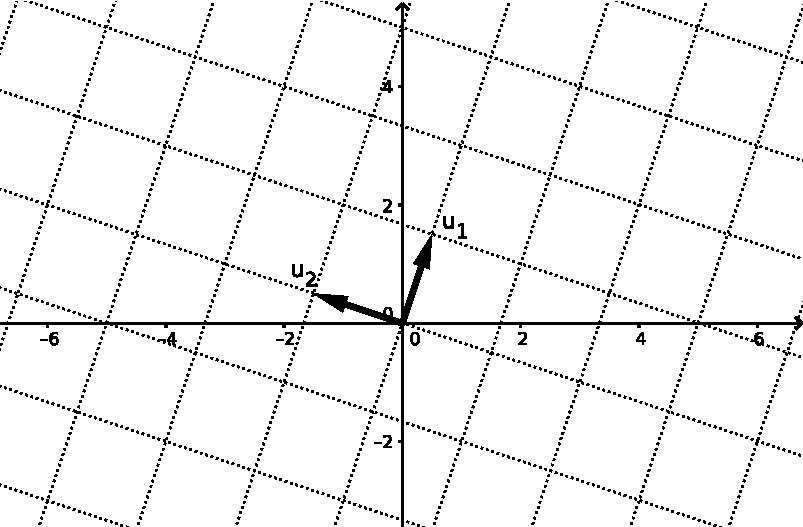
\includegraphics[width=15.0cm]{img/prova-2-nex-base-R2}
\end{center}

%\newpage
%\restoregeometry
%\section*{Respostas}
%\shipoutAnswer
\end{document}
